\documentclass[
  aps,
  reprint,
  superscriptaddress,
  floatfix,
  nofootinbib,
  longbibliography
]{revtex4-2}

\usepackage{amsmath,amssymb}
\usepackage{graphicx}
\usepackage{xcolor}
\usepackage{tikz}
\usetikzlibrary{calc,positioning,arrows.meta}
\usepackage{hyperref}

\hypersetup{
  colorlinks=true,
  linkcolor=blue,
  citecolor=blue,
  urlcolor=blue
}

% --- convenience macros -------------------------------------------------
\newcommand{\R}{\mathbb{R}}
\newcommand{\E}{\mathbb{E}}
\newcommand{\Prob}{\mathbb{P}}
\newcommand{\Sph}[1]{S^{#1}}
\newcommand{\Msem}{M}
\newcommand{\sint}{\sigma_{\mathrm{int}}}
\newcommand{\Eint}{E_{\mathrm{int}}}
\newcommand{\T}{^{\mathsf{T}}}
\newcommand{\opnorm}[1]{\lVert #1 \rVert_{\mathrm{op}}}
\newcommand{\norm}[1]{\lVert #1 \rVert}

\DeclareMathOperator*{\argmax}{arg\,max}
\DeclareMathOperator{\spanop}{span}
\DeclareMathOperator{\Var}{Var}

\begin{document}

\title{Geometric Limits on Semantic Expressibility: Quantum-Inspired Contexts and Polysemy in Large Language Models}

\author{Karl Svozil}
\email{karl.svozil@tuwien.ac.at}
\affiliation{Institute for Theoretical Physics, TU Wien (Vienna University of Technology),
Wiedner Hauptstra\ss{}e 8--10/136, 1040 Vienna, Austria}

\date{\today}

\begin{abstract}
A fixed-width language model has only $d$ independent coordinates, yet at fixed
angular tolerance it can geometrically accommodate exponentially many nearly
orthogonal feature directions.  L\'evy concentration and
Johnson--Lindenstrauss embeddings anchor this claim, but coexistence does not
guarantee cost-free simultaneous readout.  In a benchmark of uniformly random
directions, a typical pair overlaps by order $1/\sqrt d$; if both features are
active with similar strengths, an inner-product readout of either receives an
unwanted contribution about $1/\sqrt d$ times the desired signal.  Separately,
we propose for empirical testing a shared-subspace model in which different
senses reuse one token-associated component.  The construction is classical;
no experiment is reported.
\end{abstract}

\maketitle


% ======================================================================
\section{Introduction}
\label{sec:intro}
% ======================================================================

This chapter examines contextual representation in large language models
(LLMs) as part of the volume's broader inquiry into ``quantum thinking.''  A
short operational picture is enough to begin.  Text is divided into tokens;
each token is mapped to an initial vector; Transformer layers turn those
initially context-free vectors into context-dependent hidden states; and an
output map assigns probabilities to possible next tokens
\cite{Vaswani-2017-Attention}.  Section~\ref{sec:llm-loops} explains this loop
in plain language.  Appendix~\ref{app:llm-loops} gives a deliberately minimal
formal version that may be skipped on a first reading.

The central question is simple: how can a space with only $d$ independent
coordinates accommodate a much larger dictionary of approximately distinct
semantic directions, and what prevents all of them from being used at once?
The positive thesis has two parts.  High dimension makes a large dictionary
geometrically possible, but useful meaning is limited by coactivation and
readout.  Learning should therefore spend its limited angular separation where
cross-talk is costly---between important features that often activate
together.  For lexical ambiguity, a reusable token component may additionally
be shared across several low-rank sense models.

This is an analytical and model-proposal chapter; it reports no new experiment.
The geometric results are established mathematics used as null benchmarks.
The coactivation prediction and the tied shared-subspace model are empirical
hypotheses, and Sec.~\ref{sec:predictions} gives tests under which they fail.
Stating that status early is important: a possible arrangement of vectors is
not evidence that an LLM has learned that arrangement.

\paragraph{Elementary mathematical map.}
Most steps below reduce to familiar undergraduate facts.  The Pythagorean
theorem and the orthogonal projection theorem split a vector into perpendicular
components.  The Cauchy--Schwarz and triangle inequalities bound inner products
and accumulated error.  The polarization identity converts squared distances
into inner products.  The spectral theorem diagonalizes real symmetric
matrices.  Finally, additivity of variance explains root-mean-square growth,
and the union bound says that the chance of any bad event is at most the sum of
their individual chances.  The core argument uses these elementary facts.
L\'evy concentration and the Johnson--Lindenstrauss (JL) lemma are quoted;
a few explicitly optional comparisons use additional standard results and may
be skipped.

Let $d$ be the number of vectors in an orthonormal basis of the usable carrier.
It is the one exact vector-space dimension in the chapter.  Let $\Msem$ be the
measured number of feature directions returned by a declared extraction and
duplicate-removal rule.  It is a count, not a dimension.  For unit vectors,
Cauchy--Schwarz gives $|u\T v|\leq1$, and $u\T v$ is the cosine of their angle.
We call a dictionary $\varepsilon$-quasi-orthogonal when every absolute
pairwise inner product is at most the chosen tolerance
$0<\varepsilon<1$.  The function $M_\varepsilon(d)$ is the largest possible
size of such a finite code in $\R^d$; it is not a second dimension.

High-dimensional concentration and JL projection both lead to the same
single-exponential existence scale: for fixed $\varepsilon$ and sufficiently
large $d$, one can construct at least
$\exp(c\varepsilon^2d)$ quasi-orthogonal directions for some constant $c>0$.
These are related formulations of one concentration phenomenon, not two
independent capacity mechanisms.  JL preserves a prescribed finite geometry;
random spherical coding instead supplies a null distribution for a sampled
dictionary and its most extreme overlap.  A conditional double exponential
after separately assuming a fully accessible tensor-product carrier is
discussed separately in the conditional remark in
Sec.~\ref{sec:quasiortho}; it is not an LLM capacity
claim.

Geometric coexistence is only the first half of the problem.  Suppose $k$
random-like features are active together.  A simple correlation readout of one
chosen feature receives many small cross terms.  Their variances add, giving a
root-mean-square (RMS) interference scale $\sqrt{k/d}$.  This is the
Pythagorean rule applied to random errors: it describes average squared
fluctuation, not cancellation in every example.  The empirical prediction is
therefore about the placement of overlap, not merely its existence.  Important,
frequently coactive features should cause less held-out cross-talk than
activity-matched controls.

Lexical ambiguity supplies the second hypothesis.  The same token can occur in
financial, river-edge, or seat/bench uses of ``bank,'' while its surrounding
sequence drives different contextual states.  The proposal ties a
token-associated reference subspace across senses and learns separate
low-dimensional residual subspaces.  Tying pools evidence for the common
component and prevents each sense model from relearning it.  The predicted
benefit is regularization and sample efficiency, especially for rare or
imbalanced senses; with abundant data or no stable shared component, the
constraint may do nothing or may hurt.  Because every vector admits an
orthogonal decomposition, merely finding a shared component is trivial.  The
nontrivial test is incremental held-out value beyond token-mean subtraction,
top-principal-component removal, and parameter-matched unstructured models.

Current Transformers remain classical systems.  Real vectors, inner products,
high dimension, or probabilistic output do not make a computation quantum.
Here ``quantum-inspired'' refers only to a possible organization by
context-indexed projectors and symmetric operators.  The operator vocabulary
earns a specifically quantum-like role only if prespecified sequential probes
predict order effects beyond equally expressive classical baselines.  The
relation to quantum cognition and compositional distributional semantics is
reviewed in Sec.~\ref{sec:related-quantum}; no physical quantumness, Born-rule
dynamics, or semantic Kochen--Specker theorem is inferred.

A practical caveat concerns anisotropy: an LLM layer may use fewer directions
than its nominal width suggests.  Here $d$ means the \emph{usable exact
dimension} after a declared restriction or whitening rule.  By the spectral
theorem, the empirical covariance matrix has an orthonormal eigenbasis; keeping
or rescaling selected eigenvectors defines the tested carrier, and $d$ counts
those retained axes.  The resulting numerical rank is protocol-dependent, so
the selection rule must be reported.

The lexical hypothesis is intended for ambiguous tokens with established
inventories such as WordNet or OntoNotes and enough labeled contexts from
resources such as SemCor or the Word-in-Context (WiC) benchmark
\cite{pilehvar2019wic}.  It is adjacent to the superposition hypothesis in
mechanistic interpretability, according to which neural networks may represent
more features than neurons by using nonorthogonal directions with sparse
activity~\cite{elhage2022superposition}.  The present chapter separates that
global geometric background from a local, testable organization of polysemy.

The remaining sections follow the argument in that order.
Section~\ref{sec:concentration} develops the geometric null model;
Sec.~\ref{sec:dictionary-readout} turns coexistence into a readout problem;
Secs.~\ref{sec:reference} and \ref{sec:attention} present the tied
shared-subspace model and its router; and Sec.~\ref{sec:discussion} relates the
proposal to existing work, limitations, and proposed experiments.

For reference, $\R^d$ is the usable Euclidean carrier, $u\T v$ denotes the
inner product, the superscript $\mathsf T$ denotes transpose, and
$\norm{v}=\sqrt{v\T v}$.  The unit sphere is
$\Sph{d-1}=\{v\in\R^d:\norm v=1\}$; $I$ is the identity matrix;
$\Prob(A)$ is the probability of an event $A$, $\E[Y]$ is the average of a
random quantity $Y$, and
$\Var(Y)=\E[(Y-\E[Y])^2]$ is its mean squared fluctuation.  The
symbols $\approx$, $\sim$, $\lesssim$, and $\gtrsim$ below indicate scaling or
approximation at the stated level, not exact equality.  Local ranks and error
tolerances are introduced only where they are used.

% ======================================================================
\section{From text to weights and back to text: three computational loops}
\label{sec:llm-loops}
% ======================================================================

The word \emph{weight} is used for two different objects in informal accounts
of Transformers.  A trained model has persistent numerical parameters: its
embedding table, query, key, value, output, and feed-forward matrices,
normalization parameters, and final vocabulary readout.  Self-attention also
computes input-dependent coefficients that are often called attention
weights.  Those coefficients exist only for the current forward pass.  They
do not become persistent model parameters.  Keeping this distinction visible
separates the three computational loops below.

\subsection{Creating the weights: tokenization, contextual vectors, and training}
\label{sec:prose-training}

Training begins with text, but a neural network does not receive words or
sentences as primitive objects.  A tokenizer first segments character strings
into a finite vocabulary of token types and replaces each occurrence by an
integer identifier.  Tokens may be whole words, word fragments, punctuation,
spaces, or byte-level units.  Modern subword schemes are designed to cover
rare and previously unseen words without assigning a separate vocabulary
entry to every possible word~\cite{sennrich2016subword,Brown2020May}.  The
tokenizer is normally learned or chosen before the main language-model
optimization and is then held fixed during that optimization.

An embedding table associates each token identifier with an initial real
vector.  At this first lookup stage, two occurrences of the same token use the
same table entry.  Position information is also supplied, either through
added position vectors or through mechanisms such as rotary transformations
inside attention; some systems add role or segment information as well.  The
lookup vector is therefore not yet the fully contextual meaning of that
occurrence.  Context dependence is created by the successive Transformer
layers.

Within one self-attention head, the current vector at each position is mapped
by learned matrices to a query, a key, and a value.  The query at one position
is compared by an inner product with keys at other permitted positions.  In
the decoder-only autoregressive Transformer considered here, a causal mask
excludes future positions during next-token training.  Softmax normalization
turns the permitted comparisons into nonnegative attention coefficients, and
those coefficients sum to one.  The update is therefore a weighted average of
the value vectors.  Cauchy--Schwarz bounds each raw query--key comparison by the
product of the two vector lengths; the learned matrices determine which
directions make that comparison large.
Multiple heads can learn different patterns of dependence.  Residual
connections, normalization, and feed-forward blocks then transform the update
further.  After many layers, the hidden vector for an occurrence of ``bank''
can differ substantially between financial, river-edge, and seat/bench
contexts even though all occurrences began from the same token-table
entry~\cite{Vaswani-2017-Attention}.

This forward calculation still does not create new persistent weights.  The
last hidden state at each training position is converted into scores for the
next token.  The discrepancy between the predicted distribution and the
observed next token defines a training loss.  Backpropagation differentiates
that loss through the output map, feed-forward blocks, attention operations,
and embedding table.  Mathematically, backpropagation is repeated application
of the multivariable chain rule.  An optimizer then changes the persistent
parameters.
Repeating this cycle over many batches creates the trained weight values.  In
short, self-attention produces contextual activations and differentiable
routes through which error signals flow; gradient-based optimization produces
the persistent model weights~\cite{Goodfellow-et-al-2016-Book}.

Does this description require a Hilbert space?  Nothing here requires more
than finite-dimensional Euclidean inner-product geometry.  Because $\R^d$ is
complete, it may formally be called a real Hilbert space, but completeness
plays no computational role and implies no quantum mechanism.  The
construction needs ordinary real vectors, inner products, matrices, and
nonlinear maps; it does not require complex amplitudes, Born probabilities, or
quantum hardware.  Nor does training assign one exactly orthogonal vector to
every token or every meaning.  The quasi-orthogonal geometry studied later
concerns a declared dictionary of extracted feature directions at a chosen
resolution.  It is a possible organization of learned semantic distinctions,
not an assumption built into tokenization or self-attention.

\subsection{Generating an output: tokenization and autoregressive feedback}
\label{sec:prose-generation}

Response generation begins with the same tokenizer.  The prompt, including
any control, role, or formatting tokens exposed to the model, is converted to
a token sequence and then to initial vectors.  The trained parameters are now
normally fixed.  A causal forward pass produces contextual hidden states for
the prompt, and the final relevant state is mapped to one score for every
token in the vocabulary.  Softmax converts these scores into a next-token
distribution.  Greedy decoding chooses its largest entry; sampling may use a
temperature or restrict attention to a high-probability subset before drawing
a token.

The selected token is appended to the sequence.  The enlarged sequence is
then the context for the following prediction, so the generated token can
change all subsequent attention patterns and hidden states.  This loop is
repeated until an end condition is reached.  Implementations commonly cache
previous keys and values to avoid recomputing unchanged parts of the prefix,
but caching changes efficiency rather than the trained parameters.  Finally,
the tokenizer's inverse assembly rules turn the generated token identifiers
back into a character string~\cite{Brown2020May}.

Autoregressive generation is thus already recursive in a precise but limited
sense: each output token becomes part of the next input.  The context,
attention coefficients, and hidden vectors evolve from step to step, while
the persistent model weights remain fixed.  The standard decoding interface
does not require a separately represented complete answer; it emits tokens
successively by repeatedly mapping the current vector-valued context to a
distribution over the next discrete token.

\subsection{Recursive adaptation, alignment, and hallucination}
\label{sec:prose-online}

Three forms of recursion should be separated.  First, in autoregressive
generation each output token becomes part of the next input, while the model
parameters remain fixed.  Second, an external memory, retrieval result, tool
output, or longer conversation history can enlarge the next input without
changing those parameters.  Third, genuine online learning can update selected
parameters after an interaction.  Dynamic evaluation shows that the third loop
is technically possible~\cite{rannentriki2024dynamic}, but it is a separate
learning rule rather than ordinary frozen-weight inference.

This subsection is orientation only; no later geometric conclusion depends on
it.  Online learning needs verified feedback and safeguards against drift,
forgetting, poisoning, and error reinforcement.  Post-training alignment is
also a separate intervention: it changes the objective toward selected forms
of instruction following, helpfulness, and safety
\cite{ouyang2022instructgpt}.  Alignment and factual accuracy are not opposite
ends of one scale.  Preference optimization can encourage agreement in some
settings~\cite{sharma2023sycophancy}, while hallucination also occurs without
alignment~\cite{Kalai2025Why}.

Whether a particular alignment procedure increases or decreases unsupported
claims is therefore a causal question, not a consequence of the word
``alignment.''  It requires a matched control with the same base model, data
exposure, compute, prompt distribution, grounding, and decoding rule.
Appendix~\ref{app:online} gives the optional update equation, the relevant
safeguards, and this matched comparison in more detail.

% ======================================================================
\section{How high dimension supports many nearly orthogonal directions}
\label{sec:concentration}
% ======================================================================

The question is now geometric: at a fixed angular resolution, how does the
number of available directions grow with the exact carrier dimension?  Here
$d$ is the usable carrier rank, whereas $\Msem$ counts the directions in one
measured dictionary and may exceed $d$.  For a dictionary
\begin{equation}
\label{eq:quasiortho}
W=\{w_1,\ldots,w_{\Msem}\}\subset\Sph{d-1},
\qquad
\mu(W)=\max_{i\ne j}|w_i\T w_j|.
\end{equation}
For $0<\varepsilon<1$, we call this particular dictionary
$\varepsilon$-quasi-orthogonal when $\mu(W)\leq\varepsilon$, and write
$M_\varepsilon(d)$ for the maximum cardinality achievable in $\R^d$ under
this condition.  Thus
$M_\varepsilon(d)$ and the empirical count $\Msem$ are cardinalities, not
additional vector-space dimensions.  The term \emph{quasi-dimensionality}
will refer only to this resolution-dependent abundance of directions.

Two elementary facts place this definition.  Exactly orthogonal nonzero
vectors are linearly independent, so rank--nullity limits an exactly
orthogonal family to $d$ members.  Quasi-orthogonal vectors need not be
independent.  Nevertheless, $M_\varepsilon(d)$ is finite when
$\varepsilon<1$: the condition keeps every pair a fixed positive distance
apart, while the unit sphere (with opposite signs identified) is compact.  A
compact set cannot contain infinitely many points separated by the same
positive distance.  Thus this is an ordinary finite packing problem, not a new
linear dimension.

The mathematical ingredients below are established results.  L\'evy
concentration says that near-orthogonality is typical relative to a fixed
direction.  The JL lemma repackages the same high-dimensional concentration as
a finite-set projection theorem.  Direct random coding supplies a null
ensemble for the largest overlap in a sampled dictionary.  These are related
views of one phenomenon, useful for different diagnostics; their rates are not
independent effects to be multiplied.  None identifies semantic features in
an LLM.

\subsection{L\'evy concentration: why random directions are nearly perpendicular}
\label{sec:levy}

In one standard form of L\'evy's lemma, let
$f:\Sph{d-1}\rightarrow\R$ be $L$-Lipschitz: changing its input by a distance
$r$ changes its value by at most $Lr$.  If $m_f$ is a median of $f$, then, for
$t>0$,
\begin{equation}
\label{eq:levy-general}
\Prob\{|f-m_f|\geq t\}
\leq
2\exp\!\left[-c\,\frac{(d-1)t^2}{L^2}\right]
\end{equation}
for a universal constant $c>0$
\cite{ledoux2001concentration,milman1986asymptotic}.  The choice of median or
mean and the numerical constant vary among formulations; the invariant
content is exponential concentration in dimension for every Lipschitz scalar
probe at fixed $t/L$.

Fix $u\in\Sph{d-1}$ and take $f_u(x)=u\T x$.  This function is
$1$-Lipschitz because Cauchy--Schwarz gives
$|u\T(x-y)|\leq\norm{x-y}$.  By rotational symmetry it has median and mean
zero.  For
uniform $x\in\Sph{d-1}$,
\begin{equation}
\label{eq:moments}
\E[u\T x]=0,
\qquad
\Var(u\T x)=\frac{1}{d}.
\end{equation}
The variance $1/d$ is just Pythagoras plus symmetry.  Rotate coordinates so
that $u$ is the first basis vector.  Since
$x_1^2+\cdots+x_d^2=1$ on the unit sphere and the coordinates have identical
distributions, each has expected square $1/d$.  Chebyshev's inequality would
already show that large overlaps become uncommon, but only with a polynomial
bound.  L\'evy's lemma sharpens this to the exponential spherical-cap estimate
\begin{equation}
\label{eq:overlap}
\Prob\{|u\T x|\geq\varepsilon\}
\leq
2\exp\!\left[-\frac{(d-1)\varepsilon^2}{2}\right],
\qquad 0<\varepsilon<1.
\end{equation}
Thus almost every direction lies close to the equator perpendicular to a
specified direction, with a typical overlap amplitude of order
$d^{-1/2}$.

There is an equivalent angular description.  If the sign of a direction is
irrelevant, its principal angle from $u$ is
$\theta_{\rm pr}=\arccos|u\T x|$.  The first-order Taylor approximation near
zero is $\arccos z\approx\pi/2-z$, with only cubic and higher corrections, so its typical deviation from $\pi/2$ is of
order $d^{-1/2}$.  In the independently sampled isotropic null, a randomly
chosen pair therefore
exhibits \emph{angular homogenization}: its principal angle lies in a band of
width proportional to $d^{-1/2}$ near $\pi/2$ at any fixed confidence level.
Increasing the dictionary size at
fixed $d$ does not narrow this typical-pair distribution; instead it increases
the extreme overlap, as quantified below.  High dimension creates both the
typical angular concentration and room for exponentially large finite codes.

\paragraph{Optional complex comparison.}
For comparison with the later operator language, the corresponding complex
statement is especially sharp.  If $\phi,\psi$ are independent unit vectors
drawn uniformly under all unitary rotations (the meaning of ``Haar-random''), then
$Z=|\langle\phi,\psi\rangle|^2$ has the
$\operatorname{Beta}(1,d-1)$ distribution.  Using the same
$\varepsilon$ for an overlap \emph{amplitude}, rather than changing midway to
a squared-overlap tolerance, gives the exact tail
\begin{equation}
\label{eq:complex-haar-tail}
\Prob\{|\langle\phi,\psi\rangle|\geq\varepsilon\}
=(1-\varepsilon^2)^{d-1}
\leq
\exp[-(d-1)\varepsilon^2].
\end{equation}
Unitary symmetry lets us hold $\phi$ fixed as the first coordinate vector.
The squared coordinate magnitudes sum to one, the complex analogue of
Pythagoras, and integrating the first-coordinate density gives the displayed
tail.  Readers who wish to remain in real vector spaces may skip this exact
comparison; no later LLM claim depends on it.

The real and complex formulas differ in constants and exact distributions,
but both exhibit the same operative exponential scale
$\exp[-c d\varepsilon^2]$.

\subsection{Johnson--Lindenstrauss: preserving a finite cloud of points}
\label{sec:jl}

L\'evy's lemma describes most points on a sphere.  The JL lemma gives a related
finite-set formulation: a finite cloud can be compressed while all pairwise
squared distances change by at most a chosen relative error.  The surprising
feature is that the required target dimension grows only as the logarithm of
the number of points.  Specifically, for
$0<\delta<1$ and a finite set $X$, there is a linear map
$\Phi$ into $\R^d$ such that
\begin{equation}
\label{eq:jl}
\begin{aligned}
(1-\delta)\norm{x-y}^2
&\leq\norm{\Phi x-\Phi y}^2\\
&\leq(1+\delta)\norm{x-y}^2,
\qquad x,y\in X,
\end{aligned}
\end{equation}
provided
\begin{equation}
\label{eq:jl-dimension}
d\geq C_{\rm JL}\delta^{-2}\log |X|
\end{equation}
for a universal $C_{\rm JL}$~\cite{johnson-1984,Dasgupta-2003}.

To make the connection to quasi-orthogonality explicit, let $e_i$ be the
standard coordinate vector with a one in position $i$ and zeros elsewhere,
and take
\[
X=\{0,e_1,\ldots,e_{\Msem}\}\subset\R^{\Msem}.
\]
Including the origin is important: Eq.~\eqref{eq:jl} then controls both the
norms $\norm{\Phi e_i}$ and the distances
$\norm{\Phi e_i-\Phi e_j}$.  The real
polarization identity gives
\begin{equation}
\label{eq:polarization}
2(\Phi e_i)\T(\Phi e_j)
=\norm{\Phi e_i}^2+\norm{\Phi e_j}^2
-\norm{\Phi e_i-\Phi e_j}^2.
\end{equation}
This identity follows by expanding the three squared norms and cancelling
terms.  In the original set, $\norm{e_i}^2=1$ and
$\norm{e_i-e_j}^2=2$.  Because the origin was included, JL controls each
projected norm as well as each projected distance.  Substituting those bounds
into the polarization identity gives
$|(\Phi e_i)\T(\Phi e_j)|\leq2\delta$, while
$\norm{\Phi e_i}^2\geq1-\delta$.  After normalization,
$w_i=\Phi e_i/\norm{\Phi e_i}$, one obtains
\begin{equation}
\label{eq:jl-coherence}
|w_i\T w_j|
\leq\frac{2\delta}{1-\delta}
\qquad(i\ne j).
\end{equation}
Normalization divides by
$\norm{\Phi e_i}\norm{\Phi e_j}\geq1-\delta$, which explains the denominator.
Taking $\delta=\varepsilon/(2+\varepsilon)$ makes the right-hand side of
Eq.~\eqref{eq:jl-coherence} equal to $\varepsilon$.  Reading
Eq.~\eqref{eq:jl-dimension} constructively therefore gives, for every fixed
$0<\varepsilon<1$ and all sufficiently large $d$,
\begin{equation}
\label{eq:jl-inverse}
M_\varepsilon(d)
\geq
\exp(c'\varepsilon^2d),
\end{equation}
for a universal $c'>0$.  This is an existence lower bound.  Sharp lower bounds for worst-case JL
dimension reduction~\cite{alon2016optimal,larsen-nelson-2017} do not, by
themselves, establish a matching universal upper bound for spherical codes,
and no such upper bound is claimed here.  Algebraically, the exponential
appears simply by solving the logarithmic dimension condition for the number
of points: undoing a logarithm requires exponentiation.

\subsection{Direct random coding and the Welch floor}
\label{sec:quasiortho}

The exponential scale can also be reached directly.  Draw the $\Msem$
directions independently from the uniform measure on $\Sph{d-1}$.  Applying
Eq.~\eqref{eq:overlap} to all unordered pairs gives
\begin{equation}
\label{eq:unionbound}
\Prob\{\mu(W)\geq\varepsilon\}
\leq
\Msem(\Msem-1)
\exp\!\left[-\frac{(d-1)\varepsilon^2}{2}\right].
\end{equation}
There are $\binom{\Msem}{2}$ unordered pairs.  The union bound says that the
probability that at least one pair is bad is no larger than the sum of the
individual bad-pair probabilities; the pair events need not be independent.
The factor two in Eq.~\eqref{eq:overlap} cancels the factor one-half in the
number of pairs.
Whenever the right-hand side is less than one, at least one
$\varepsilon$-quasi-orthogonal dictionary must exist: failure cannot occur for
every random draw.  This is the elementary probabilistic method.  It
reproduces the $\exp(c\varepsilon^2d)$ lower scale through the same underlying
concentration mechanism as JL, now as an ensemble calculation rather than a
finite-metric projection statement.  The two rates must not be multiplied or
counted as independent amplifications.  Equation~\eqref{eq:unionbound} is only
a sufficient random-code bound; it is neither an optimized-code upper bound
nor a semantic capacity theorem.

Equating the number of pairs to the real spherical-cap tail gives the useful
finite-sample null estimate
\begin{equation}
\label{eq:max-overlap}
\mu_{\max}^{\rm null}(d,\Msem)
\approx
2\sqrt{\frac{\log\Msem}{d}},
\qquad
\log\Msem\ll d,
\end{equation}
up to lower-order spherical-cap factors.
The estimate comes from setting the right-hand side of the union bound to a
number of order one.  Taking logarithms turns a product into a sum, and solving
$\Msem^2\exp(-d\varepsilon^2/2)\approx1$ for $\varepsilon$ gives the displayed
square root.  It is therefore an extreme-value calibration for a random
ensemble.  It describes the most extreme pair
in an independently sampled isotropic dictionary, not the overlap of a
typical pair and not a hard limit on a learned one.

A genuine deterministic restriction is supplied by the Welch bound:
\begin{equation}
\label{eq:welch}
\mu(W)^2
\geq
\frac{\Msem-d}{d(\Msem-1)}
\qquad(\Msem>d),
\end{equation}
for every unit-vector dictionary~\cite{welch1974coherence}.  The Welch floor,
the random maximum in Eq.~\eqref{eq:max-overlap}, and the existence lower
bound in Eq.~\eqref{eq:jl-inverse} answer different questions and should not
be presented as the two edges of one universal interval.

The Welch bound itself follows from familiar linear algebra.  Form the Gram
matrix $G=(w_i\T w_j)_{i,j}$, whose entries are all pairwise inner products.  It is
positive semidefinite, has rank at most $d$, and has trace $\Msem$.  By the
spectral theorem it has at most $d$ nonzero eigenvalues, and Cauchy--Schwarz
says that the sum of their squares is at least $\Msem^2/d$.  The diagonal of
$G$ already contributes $\Msem$ to that sum of squares.  The average squared
off-diagonal entry must therefore be at least the right-hand side of
Eq.~\eqref{eq:welch}; the maximum cannot be smaller than the average.

\paragraph{Optional complex code.}
The exact complex-Haar law in Eq.~\eqref{eq:complex-haar-tail} makes the
corresponding random-code statement particularly transparent.  If
$M_\varepsilon^{\mathbb C}(d)$ denotes the maximum cardinality in
$\mathbb C^d$ at the same amplitude tolerance, a union bound over all pairs
gives the explicit existence result
\begin{equation}
\label{eq:complex-code}
M_\varepsilon^{\mathbb C}(d)
\geq
\left\lfloor
\exp\!\left[
\frac{d-1}{2}\bigl(-\log(1-\varepsilon^2)\bigr)
\right]
\right\rfloor .
\end{equation}
This is the sharper complex analogue of the real exponential scale, not an
additional linear dimension.

\paragraph{Conditional tensor-product remark (not an LLM capacity claim).}
The conditional double exponential requires two separate steps.  If
an independently justified carrier is the full tensor product
$\bigotimes_{a=1}^{n}\R^q$, with fixed $q>1$, then its exact dimension is
\begin{equation}
\label{eq:product-dimension}
d=q^n.
\end{equation}
The elementary tensor-product basis is indexed by $n$ independent choices,
each with $q$ possibilities, so the multiplication principle gives $q^n$
basis vectors.  Quasi-orthogonal coding is then exponential in that already
exponential dimension.
For fixed $0<\varepsilon<1$, substitution into Eq.~\eqref{eq:jl-inverse} gives
\begin{equation}
\label{eq:double-quasi}
M_\varepsilon(q^n)
\geq
\exp\!\bigl(c'\varepsilon^2q^n\bigr),
\end{equation}
which is doubly exponential in $n$.  Equation~\eqref{eq:complex-code} gives
the same conclusion, with an explicit exponent, for a full complex
tensor-product carrier.  These bounds concern arbitrary directions in the
full carrier.  They do not follow if admissible states are restricted to
product vectors or another low-complexity manifold; access to the full carrier,
or a code construction within the admissible class, is an additional premise.
An ordinary Transformer residual stream is presented only as a measured real
carrier $\R^d$.  Its width, layers, heads, or token positions do not by
themselves establish independent semantic tensor factors.  For an LLM the
unconditional geometric statement is therefore an existence lower bound
exponential in the declared usable $d$; Eq.~\eqref{eq:double-quasi} is a
further tensor-product hypothesis, not an architectural consequence.  No later semantic conclusion in this
chapter depends on this remark.

% ======================================================================
\section{From geometric coexistence to semantic readout}
\label{sec:dictionary-readout}
% ======================================================================

An exponential dictionary can coexist geometrically without all its
coefficients being simultaneously accessible.  Readout depends on which
directions activate together, their amplitudes, the decoder, and the required
error probability.  This distinction is where the geometry acquires
potential semantic content.

\subsection{Fixed-target, worst-case, and joint readout}

Let an active set $S$ of size $k$ produce the hidden state
\begin{equation}
\label{eq:hidden}
h=\sum_{j\in S}x_jw_j .
\end{equation}
Here $S$ is the set of features active in this example, $k=|S|$, and $x_j$
is the amplitude of feature $j$.  This is simply a linear combination of the
active directions.
For one specified active target $i\in S$, a correlation decoder returns
\begin{equation}
\label{eq:readout}
w_i\T h
=x_i+
\sum_{\substack{j\in S\\j\ne i}}
x_jw_i\T w_j.
\end{equation}
This identity uses only distributivity of the inner product and
$w_i\T w_i=1$.  The first term is the desired signal; every cross inner
product in the remaining sum is interference.
In the exact independently sampled isotropic ensemble, provided $S$ and the
amplitudes are fixed or selected independently of the direction draws,
conditional on $S$, $(x_j)$, and $w_i$, the variables $w_i\T w_j$ for $j\ne i$
are independent, centered, and have variance $1/d$.  Consequently
\begin{equation}
\label{eq:intvar}
\Var\!\left[
\sum_{\substack{j\in S\\j\ne i}}
x_jw_i\T w_j
\;\middle|\;S,(x_j),w_i
\right]
=
\frac{1}{d}
\sum_{\substack{j\in S\\j\ne i}}x_j^2 .
\end{equation}
For independent centered random terms, covariance terms vanish, so the
variance of a sum is the sum of the variances.  This is the probabilistic
version of Pythagoras.  It describes average squared fluctuation and does not
assert cancellation in each individual context.
For a learned, merely random-like dictionary this equality is used only as an
approximate null calibration.  For comparable order-one amplitudes it gives
the fixed-target RMS scale
\begin{equation}
\label{eq:sint}
\sint
\sim\sqrt{\frac{k-1}{d}}
\approx\sqrt{\frac{k}{d}}.
\end{equation}
This estimate is a property of the declared correlation decoder under
cancellation assumptions, not a universal recovery law.

Without cancellation, coherence yields the deterministic target-wise bound
\begin{equation}
\label{eq:worst-readout}
|w_i\T h-x_i|
\leq
\mu(W)\sum_{\substack{j\in S\\j\ne i}}|x_j|.
\end{equation}
This bound follows from the triangle inequality and
$|w_i\T w_j|\leq\mu(W)$.  Unlike the RMS estimate, it assumes no cancellation,
so the possible error grows linearly with the absolute amplitudes.
The distinction becomes sharper for joint recovery.  With $W_S$ the matrix
whose columns are the active directions, let $x_S$ collect their amplitudes and
let $\widehat{x}_S$ collect their correlation readouts.  With
$G_S=W_S\T W_S$, simultaneous readout gives
\begin{equation}
\label{eq:joint-readout}
\widehat{x}_S
=W_S\T h
=G_Sx_S,
\qquad
\opnorm{G_S-I}
\leq(k-1)\mu(W),
\end{equation}
where $\opnorm{A}$ is the operator norm, the largest factor by which $A$ can
stretch a unit vector.  The last inequality follows, conservatively, from
Gershgorin's theorem.
The Gram matrix has ones on its diagonal and pairwise overlaps off the
diagonal.  Gershgorin's theorem says that each eigenvalue lies within an
off-diagonal row sum of a diagonal entry; here that row sum is at most
$(k-1)\mu(W)$.  If it is below one, $G_S$ is invertible and coefficients on a
known support can be recovered by applying $G_S^{-1}$.  If $k>d$, rank--nullity
instead makes $G_S$ singular.
Support identification must additionally control false readouts among the
$\Msem-k$ inactive directions, introducing a multiple-comparison cost.
Uniform recovery of every sparse coefficient vector is therefore a stronger
problem than the fixed-target calculation above: it requires additional
assumptions and is not implied by the coherence or JL statements.  We do not
use such a uniform-recovery theorem here.
The exponential coexistence of directions, fixed-target RMS access, worst-case
access, and joint coefficient recovery are four distinct statements.

\subsection{Why semantic interference must be conditioned on coactivation}
\label{sec:coactivation-diagnostic}

Maximum coherence assigns the same cost to every pair.  A semantic decoder
does not: two directions that never activate together can overlap without
contributing to the error in Eq.~\eqref{eq:readout}.  Conversely, even a
moderate overlap can be expensive when the pair coactivates often, carries
large amplitudes, and matters to the task.  Define the ordered, nonnegative
activity-and-importance weight
\begin{equation}
\label{eq:coactivation}
a_{ij}
:=
\omega_i\,\E\!\left[
\mathbf 1_{\{i,j\ {\rm active}\}}x_j^2
\right],
\qquad \omega_i\geq0,
\end{equation}
where $\omega_i$ is a nonnegative scalar recording the task importance of accurately reading feature
$i$.  The indicator $\mathbf 1$ equals one when both features are active and
zero otherwise.  Thus $a_{ij}$ is the importance of reading $i$, multiplied by
the average squared amplitude of $j$ on examples where the pair coactivates;
it vanishes when they never coactivate.  For a fixed target $i$, write the
contribution from feature $j$ as
$c_{ij}=\mathbf 1_{\{i,j\ {\rm active}\}}x_j(w_i\T w_j)$.
If distinct contributions have zero cross-moments on the held-out distribution,
$\E[c_{ij}c_{ij'}]=0$ for $j\ne j'$, then the diagonal part of the expected
importance-weighted squared error is
\begin{equation}
\label{eq:int-energy}
\Eint
=
\sum_{i\ne j}
a_{ij}(w_i\T w_j)^2.
\end{equation}
Squaring the interference sum produces diagonal terms with the same feature
index and cross terms with two different indices.  Equation
\eqref{eq:int-energy} keeps the diagonal part; the cross terms vanish only
under the stated zero-cross-moment assumption.
We use $\Eint$ as a coactivation-weighted diagonal interference proxy.  Without
that assumption, the full squared error also contains cross-moment terms
involving distinct $j$ and $j'$.  If the contributions are centered, these
cross-moments are covariances.

This changes the scientific prediction.  A useful learned dictionary need
not beat the isotropic null on every pair, and a nonzero overlap is not itself
a defect.  If training is pressured to reduce semantic readout error, then
important, frequently coactive pairs should contribute less to
Eq.~\eqref{eq:int-energy} than they do in controls matched for $d$, $\Msem$,
marginal activity, amplitude, and feature importance.  That conditional
redistribution, not overcompleteness alone, is testable.

This prediction extends rather than replaces earlier toy-model work on
superposition, where correlated and anticorrelated features can favor different
learned geometries~\cite{elhage2022superposition}.  The additional proposal
here is the held-out, task-weighted statistic in Eq.~\eqref{eq:int-energy} for
extracted contextual features.  The general observation that feature
correlation affects packing is not claimed as new.

\subsection{A task-dependent operating window}
\label{sec:operating-criterion}

There is no task-independent numerical bracket whose lower edge is $d$ and
whose upper edge is a universal packing capacity.  A meaningful operating
window is instead the intersection of an empirical coverage requirement with
declared readout tolerances.  Let $\varepsilon_{\rm task}$ be the largest
tolerated absolute pairwise overlap for a chosen diagnostic and let $\Delta$ be the
tolerated fixed-target RMS interference.  For the real isotropic null,
Eqs.~\eqref{eq:max-overlap} and \eqref{eq:sint} give the separate crossover
scales.  They come from elementary algebra: set the random maximum
$2\sqrt{\log\Msem/d}$ equal to $\varepsilon_{\rm task}$, and set the RMS
interference $\sqrt{k/d}$ equal to $\Delta$.  Solving for the two counts gives
\begin{equation}
\label{eq:dual}
M_{\rm crowd}(d,\varepsilon_{\rm task})
\approx
\exp\!\left(\frac{d\varepsilon_{\rm task}^2}{4}\right),
\qquad
k_{\rm rms}(d,\Delta)
\lesssim d\Delta^2.
\end{equation}
The first approximation assumes the same small-overlap regime used in
Eq.~\eqref{eq:max-overlap}.  The symbols $\approx$ and $\lesssim$ mark design
scales, not sharp universal inequalities.
The first concerns the worst of order $\Msem^2$ pairs formed from $\Msem$
independently sampled directions; the second concerns one specified target
among $k$ active directions.
Let $M_{\rm req}({\cal T})$ be the smallest measured dictionary size that
reaches a prespecified coverage or performance level on task ${\cal T}$, and
let $E_{\max}({\cal T})$ be its allowed value of the interference proxy.  A
useful task-conditioned summary is
\begin{equation}
\label{eq:gold-task}
\begin{aligned}
M_{\rm req}({\cal T})&\leq \Msem,
&\mu(W)&\leq\varepsilon_{\rm task},\\
k&\lesssim k_{\rm rms}(d,\Delta),
&\Eint&\leq E_{\max}({\cal T}).
\end{aligned}
\end{equation}
Read from left to right, the display says: retain enough directions to cover
the task; require the measured worst pairwise overlap to stay below its chosen
tolerance; activate only as many directions as the RMS budget permits; and
keep measured coactivation-weighted error below its task budget.  Only the
coverage threshold comes from semantic performance.  The others are declared
geometric or readout criteria.
The scale $M_{\rm crowd}$ in Eq.~\eqref{eq:dual} remains an isotropic-null
diagnostic, not a substitute for measuring $\mu(W)$ and not a universal
spherical-code upper bound.  A learned dictionary can lie beyond that random
scale and still satisfy the declared overlap tolerance.  A stricter
joint-recovery criterion may replace the fixed-target condition through
Eq.~\eqref{eq:joint-readout}.  The Goldilocks region is thus the set of
dictionaries that provide enough measured task coverage while satisfying
explicitly selected pairwise, active-set, and readout-error criteria.  Its
lower edge comes from the task's coverage curve, not from an orthogonality
count.

For scale, if $d=4096$ and $\Msem=10^4$, Eq.~\eqref{eq:max-overlap} predicts a
random-dictionary maximum of about $9.5\%$, although one typical pair has RMS
overlap only $1/\sqrt d\approx1.6\%$.  Separately, $k=64$ gives the
fixed-target scale $\sqrt{k/d}=0.125$.  These numbers illustrate why the
dictionary count, the most extreme pair, and simultaneous readout cannot be
collapsed into one effective dimension.

Nothing in these benchmarks is specifically semantic until a feature
extractor, activity distribution, decoder, and task are fixed.  The next
section adds a separate and stronger hypothesis about how context-dependent
readout may be organized for lexically ambiguous tokens.

% ======================================================================
\section{A shared-subspace model of lexical ambiguity}
\label{sec:reference}
% ======================================================================

The previous section supplied classical geometric benchmarks.  It did not
imply any particular organization of lexical ambiguity.  We now propose a
separate classical model: occurrences of one token may share a reusable
low-dimensional component, while context-specific variation occupies residual
subspaces.  The shared part can represent lexical identity, morphology, or a
token-specific baseline.  Tying it across senses pools training examples and
reduces the number of separately estimated directions.  The expected advantage
is therefore regularization and sample efficiency, not greater expressivity.
It should be largest for rare or imbalanced senses and can disappear or reverse
when no stable shared component exists.

This supplies a possible bridge from global quasi-dimensionality to local
meaning.  A linguistic context does not decode the entire feature dictionary;
it selects a small active set or low-dimensional subspace.  The model below
organizes that selection by sharing a token-associated subspace while placing
sense-specific content in perpendicular residual subspaces.  The global code
size and this local organization are independent claims.

Fix one layer $\ell$ and one centered or whitened carrier for each test.  The
observed sequence context is $x$, while $s$ denotes only the discrete operator
class that indexes a candidate filter.  In supervised experiments an operator
class may be aligned with a labeled word sense; in unsupervised experiments it
is latent.  We abbreviate $h_\ell(t\mid x)$ by $h(x)$ when $t$ and $\ell$ are
fixed.  The notation distinguishes mathematical types and roles:
%
\begin{itemize}
\item $r_t\in\R^d$ is a unit candidate token reference vector;
\item $\mathcal R_t\subset\R^d$ is the token reference subspace;
\item $P_t$ is the orthogonal projector onto $\mathcal R_t$;
\item $S_{t,s}\subset\mathcal R_t^\perp$ is a low-dimensional sense
subspace;
\item $u_{t,s,j}\in S_{t,s}$ are vectors spanning that sense subspace;
\item $h_\ell(t\mid x)\in\R^d$ is an observed contextual hidden state.
\end{itemize}
%
Thus $r_t$, $u_{t,s,j}$, and $h_\ell(t\mid x)$ are vectors, whereas
$\mathcal R_t$ and $S_{t,s}$ are subspaces. The $w_i$ used in
Sec.~\ref{sec:concentration} have a separate role: they are generic feature
directions in the geometric null model and are not reused as sense labels.
This section resets the symbol $x$: it now denotes sequence context, not the
random point on a sphere used in Sec.~\ref{sec:levy}.

If $\mathcal R_t$ has an orthonormal basis collected in a matrix $Q_t$ with
$p$ columns, then $\mathcal R_t^\perp=\ker(Q_t\T)$.  Rank--nullity gives
$\dim(\mathcal R_t^\perp)=d-p$.  Thus every vector in a sense subspace is
perpendicular to every reference direction; no new ambient dimension is being
introduced.

\subsection{The reference-subspace hypothesis}
\label{sec:reference-hypothesis}

In the simplest version, let $r_t$ be a candidate unit direction and set
%
\begin{equation}
\label{eq:reference-direction}
\mathcal R_t=\spanop\{r_t\}.
\end{equation}
%
Empirically, $r_t$ could be a normalized mean contextual embedding, a learned
token-specific probe direction, or a static input embedding after an explicit
map into the same layer carrier. It is simply a hypothesized context-stable reference for token
identity. It is not a mechanical or dynamical object.
Any state can be decomposed relative to any direction, so the decomposition
alone has no empirical content.  This is the orthogonal projection theorem:
for every chosen subspace, each vector has a unique closest component inside
the subspace and a perpendicular residual.  A weak ``token component exists''
test is also likely to pass simply because contextual states retain token
identity.  The substantive claim is that a subspace fixed from training data
exposes additional held-out sense structure beyond token-mean subtraction,
top-principal-component removal, and matched control subspaces.

For each operator class $s$, define a low-dimensional sense subspace of rank
$m_s$
%
\begin{equation}
\label{eq:sense-subspace}
\begin{aligned}
S_{t,s}&=\spanop\{u_{t,s,1},\dots,u_{t,s,m_s}\},\\
S_{t,s}&\subset\mathcal R_t^\perp,
\qquad m_s\ll d-\dim(\mathcal R_t) .
\end{aligned}
\end{equation}
%
For the intended three-arm example, finance, river-edge, and seat/bench
associations of ``bank'' correspond to different subspaces
$S_{\mathrm{bank},s}$ inside the common orthogonal carrier
$\mathcal R_{\mathrm{bank}}^\perp$.  The verbal use in which an aircraft
banks or tilts supplies a fourth sense and would add a fourth sense
subspace; it is mentioned here but omitted from the drawing for clarity.  A
word sense is not a single vector: topic, syntax, selectional preferences,
and world knowledge may require several spanning directions $u_{t,s,j}$.

The reference object may itself require more than one direction. In that
case define
%
\begin{equation}
\label{eq:reference-subspace}
\mathcal R_t=
\spanop\{r_{t,1},\dots,r_{t,p}\},
\qquad p\ge1,
\end{equation}
%
and require
%
\begin{equation}
\label{eq:multi-sense-subspace}
S_{t,s}\subset\mathcal R_t^\perp .
\end{equation}
%
Equation~\eqref{eq:reference-direction} is the special case $p=1$.
Here $p$ is the local rank of the reference subspace; it is not another global
dimension.  The same orthogonal-projection construction works for any declared
$p$, which is why held-out comparison rather than existence carries the
scientific burden.
The bare subspace construction specifies only a pattern of sharing. In
quantum logic, different contexts can share one or more observables or
spectral projections; finite-dimensional examples with two shared
observables are known~\cite{svozil:040102}. In the semantic model,
$\mathcal R_t$ is a common token-associated reference subspace, while the
sense-specific subspaces lie in its orthogonal complement. These incidence
relations alone imply neither noncommutativity nor quantum probability. The
next subsection makes the stronger, optional operator structure explicit.

The low-rank assumption is empirical.  Tying $\mathcal R_t$ across classes
prevents each class model from independently relearning the proposed common
component.  This predicts steeper learning curves when examples per sense are
scarce and a shared component is real; an unconstrained model should catch up
with abundant data, and tying may hurt if the assumption is false.  It also predicts that dominant
within-sense variation is low-dimensional after projection onto
$\mathcal R_t^\perp$. This is compatible with evidence that contextualized
embeddings can separate word senses, but it is stronger: it asks whether
such separation is privileged relative to a token-associated reference
subspace~\cite{wiedemann2019does,scarlini2020ares}.

\subsection{Classical projectors and optional observable notation}
\label{sec:observables}

The shared-subspace hypothesis can be parameterized by a constrained family
of class-conditioned projectors.  Let $Q_t\in\R^{d\times p}$ have orthonormal columns
spanning $\mathcal R_t$, so that $P_t=Q_tQ_t\T$.  For each class $s$, let
$B_{t,s}\in\R^{d\times m_s}$ have orthonormal columns spanning $S_{t,s}$.
Here $Q_t$ and $B_{t,s}$ are basis matrices, not additional semantic
directions.  The vector $Q_t\T h$ contains the ordinary coordinates of $h$ in
the reference basis, and $Q_tQ_t\T h$ reconstructs its orthogonal projection.

The projector onto the token-plus-sense subspace is
%
\begin{equation}
\label{eq:context-projector}
\Pi_{t,s}=P_t+B_{t,s}B_{t,s}\T .
\end{equation}
Because the two bases are orthonormal and perpendicular, their cross products
vanish.  Squaring $\Pi_{t,s}$ therefore returns $\Pi_{t,s}$ itself.  This
idempotence is the defining property of the orthogonal projector onto the
direct sum $\mathcal R_t\oplus S_{t,s}$.
%
All $\Pi_{t,s}$ have the common invariant sector $\mathcal R_t$ and differ on
their sense sectors.  In particular,
%
\begin{equation}
\label{eq:projector-commutator}
[\Pi_{t,s},\Pi_{t,s'}]
=
[B_{t,s}B_{t,s}\T,B_{t,s'}B_{t,s'}\T]
\end{equation}
%
need not vanish.  The commutator is $[A,B]=AB-BA$.  Expanding both products
makes every term containing $P_t$ vanish because the sense vectors lie in
$\mathcal R_t^\perp$.  A nonzero remainder means that applying two sense
projections in opposite orders can give different vectors.  Crucially,
sharing a sector does not cause this order dependence.  Moreover, two
generic fitted projectors will often fail to commute, so a nonzero commutator
alone is not evidence for a quantum-inspired account.  It becomes
discriminating only if its size predicts an independently specified
order-sensitive contextual task or improves held-out prediction relative to
matched projector models.

\paragraph{Optional observable notation.}
The real spectral theorem says that every symmetric matrix has an orthonormal
eigenbasis.  Borrowing quantum terminology, a symmetric class ``observable''
with the same basis-independent shared sector can be written
%
\begin{equation}
\label{eq:context-observable}
A_{t,s}
=\lambda_t P_t
 +B_{t,s}\Lambda_{t,s}B_{t,s}\T,
\end{equation}
%
where the scalar $\lambda_t$ is shared across classes and the diagonal
$\Lambda_{t,s}$ is class-specific.  In the orthonormal eigenbasis,
$A_{t,s}$ assigns $\lambda_t$ to every vector in $\mathcal R_t$, assigns the
diagonal entries of $\Lambda_{t,s}$ to the chosen sense directions, and acts
as zero on the displayed remainder.  If $P_t$ is to be the spectral projector
for the shared eigenvalue, assume that $\lambda_t$ is distinct from zero and
from every diagonal entry of every $\Lambda_{t,s}$, as well as from the spectra
of any added complementary terms.  If $p>1$, $\lambda_t$ is deliberately
degenerate within $\mathcal R_t$, so the observable identifies the shared
subspace rather than an arbitrary basis within it.  Additional orthogonal
spectral terms may resolve that complement into further outcomes.  The projector
family is the empirical core of the proposal; the eigenvalues add scientific
content only if they are prespecified or learned and improve a held-out
observable outcome, rather than being assigned after the geometry is known.

The corresponding class-conditioned projection is concrete:
%
\begin{equation}
\label{eq:observable-embedding}
h_{t,s}^{(\Pi)}(x)
=\Pi_{t,s}h(x)
=P_t h(x)+B_{t,s}B_{t,s}\T(I-P_t)h(x).
\end{equation}
%
For $h(x)\ne0$, make the observable operational through its normalized
quadratic expectation and filtered state:
\begin{equation}
\label{eq:observable-readout}
o_{t,s}(x)=
\frac{h(x)\T A_{t,s}h(x)}{\norm{h(x)}^2},
\qquad
h_{t,s}^{(A)}(x)=A_{t,s}h(x).
\end{equation}
The first quantity is a Rayleigh quotient.  In the eigenbasis supplied by the
spectral theorem it is a weighted average of the eigenvalues, with weights
equal to squared coordinates of $h(x)$.  The filtered vector instead rescales
each eigencomponent.  Readers interested only in the classical projector
model may omit $A_{t,s}$ and use $\Pi_{t,s}$ throughout.
The router may use $o_{t,s}$ as a score, and a fitted module may use either
$h_{t,s}^{(\Pi)}$ or $h_{t,s}^{(A)}$ as its class-conditioned representation.
One may select a single $s$, or take a soft mixture of these outputs as in
Sec.~\ref{sec:attention}.  Equations~\eqref{eq:context-projector}--
\eqref{eq:observable-readout} define a proposed constrained module or probe;
they do not claim that current LLMs already implement it.  Quantum-logic
discussions sometimes call contexts with shared outcomes \emph{intertwining}
or interlocking.  Here ``shared-sector'' names that incidence pattern while
avoiding confusion with the operator-theoretic assertion that an intertwiner
$X$ satisfies $AX=XB$.
Everything here uses ordinary real matrices on classical hardware.

\subsection{Projection energy and subspace readout}
\label{sec:gated}

Let $h(x)\in\R^d$ be a contextual state and retain the orthogonal projector
$P_t$ defined above. The two components are
%
\begin{align}
\label{eq:reference-decomp}
h(x)&=h_{\rm ref}(x)+h_\perp(x),\\
h_{\rm ref}(x)&=P_t h(x),\nonumber\\
h_\perp(x)&=(I-P_t)h(x)\in\mathcal R_t^\perp.\nonumber
\end{align}
%
The orthogonal projection theorem makes this decomposition unique:
$P_th$ is the closest vector in $\mathcal R_t$ to $h$, and $(I-P_t)h$ is
perpendicular to that subspace.  Pythagoras gives
$\norm h^2=\norm{P_th}^2+\norm{(I-P_t)h}^2$.
The hypothesis is that most sense-disambiguating variation is present in
$h_\perp(x)$, not that the decomposition itself is special.  A
basis-invariant score can be expressed directly with the orthonormal matrices
already defined:
%
\begin{align}
\label{eq:sense-coordinates}
e_t(x)&=\norm{Q_t\T h(x)}^2=\norm{P_t h(x)}^2,\nonumber\\
\beta_{t,s}(x)&=B_{t,s}\T h_\perp(x),\\
f_{t,s}(x)&=\norm{\beta_{t,s}(x)}^2
=\norm{B_{t,s}B_{t,s}\T h_\perp(x)}^2.\nonumber
\end{align}
%
The entries of $Q_t\T h$ and $B_{t,s}\T h_\perp$ are ordinary coordinates in
orthonormal bases.  Parseval's identity says that the sum of their squared
coordinates equals the squared length of the corresponding orthogonal
projection.  This is why the energies do not depend on the particular
orthonormal basis chosen inside the same subspace.
Here $e_t$ measures energy in the candidate reference subspace and $f_{t,s}$
measures projection energy in the candidate sense subspace.  Both definitions
work for any reference rank $p$ and are invariant under changes of orthonormal
basis within either subspace.  An illustrative projection-energy score is
%
\begin{equation}
\label{eq:sense-score}
\gamma_{t,s}(x)=\frac{f_{t,s}(x)}{m_s}.
\end{equation}
%
The division by the subspace rank matters when the $m_s$ differ: for an
isotropic residual, expected raw projection energy is proportional to rank.
With equal ranks it does not change the ordering.  A more careful empirical
implementation may instead calibrate each raw energy against its own held-out
null distribution.
The selected sense label is
%
\begin{equation}
\label{eq:selected-sense}
s^*(x)=\argmax_s \gamma_{t,s}(x).
\end{equation}
%
Multiplying every $\gamma_{t,s}$ by the same positive function of $e_t$ would not
change this ranking; reference energy can instead supply an independently
calibrated engagement or abstention threshold.  The score is an illustrative
probe, not a derivation of how an LLM
must disambiguate.  At test time the true sense label is unavailable, so a
practical implementation must learn the router from context without oracle
access.  The empirical content is the proposed separation of roles: the
reference component tracks token identity or engagement, while the orthogonal
component contains sense-disambiguating information. If no token-associated
$\mathcal R_t$ exposes sense structure better than centered, token-mean,
frequency-controlled, layer-matched, and random controls, the hypothesis
fails.

Figure~\ref{fig:reference-subspace} illustrates these objects as an abstract
hypergraph incidence structure.

\begin{figure}[t]
\centering
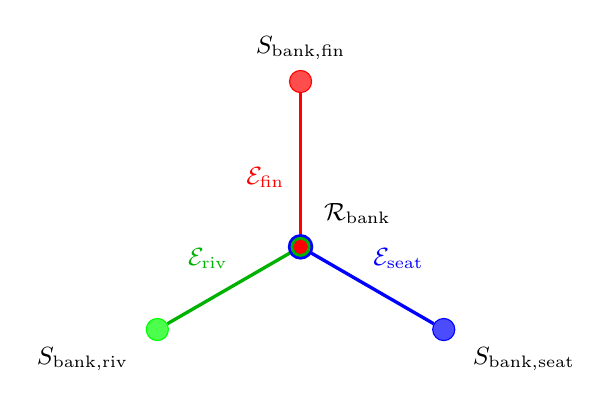
\begin{tikzpicture}[scale=0.5,
    outer/.style={circle, draw, minimum size=8pt,
                  inner sep=0pt, font=\footnotesize},
    lab/.style={font=\small}]
% central shared reference-subspace vertex
\coordinate (c) at (0,0);

\node[lab, above right=7pt] at (c)
{$\mathcal R_{\rm bank}$};

% outer sense-subspace vertices
\node[outer, red, fill=red!70,
      label={[lab]above:
      $S_{{\rm bank},{\rm fin}}$}]
      (fin) at (90:4.2cm) {};

\node[outer, green, fill=green!70,
      label={[lab, xshift=-4pt]below left:
      $S_{{\rm bank},{\rm riv}}$}]
      (riv) at (210:4.2cm) {};

\node[outer, blue, fill=blue!70,
      label={[lab, xshift=4pt]below right:
      $S_{{\rm bank},{\rm seat}}$}]
      (seat) at (330:4.2cm) {};

% hyperedges labelled by context
\draw[very thick, red] (c) --
      node[lab, left=2pt, pos=0.45]
      {$\mathcal E_{\rm fin}$} (fin);

\draw[very thick, green!70!black] (c) --
      node[lab, above left=1pt, pos=0.45]
      {$\mathcal E_{\rm riv}$} (riv);

\draw[very thick, blue] (c) --
      node[lab, above right=1pt, pos=0.45]
      {$\mathcal E_{\rm seat}$} (seat);

% central concentric disks
\filldraw[blue, very thick] (c) circle (8pt);
\filldraw[green!70!black, very thick] (c) circle (6pt);
\filldraw[red, very thick] (c) circle (4pt);
\end{tikzpicture}
\caption{%
Incidence schematic for the lexically ambiguous token ``bank.''  The center is
the single shared reference-subspace vertex
$\mathcal R_{\rm bank}$ and the outer nodes are the financial, river-edge,
and seat/bench sense subspaces in $\mathcal R_{\rm bank}^{\perp}$.  Each
colored arm denotes the displayed two-vertex fragment
$\mathcal E_s=\{\mathcal R_{\rm bank},S_{{\rm bank},s}\}$ associated with
$\Pi_{{\rm bank},s}$; it is not a vector, map, or causal arrow.  The concentric
colors at the center mark membership of the same shared vertex in all three
displayed context-hyperedge fragments.  Additional outcome sectors would
complete each measurement context in a full contextuality hypergraph.
}
\label{fig:reference-subspace}
\end{figure}

\subsection{Relation to dynamic contextual embeddings}
\label{sec:dynamic}

Transformers already handle lexical ambiguity dynamically. The hidden state
$h_\ell(t\mid x)$ of token $t$ at layer $\ell$ depends on context $x$.
The reference-subspace and shared-sector operator hypotheses are not
alternative hardware architectures; they are proposed organizations and
readouts of these observed trajectories.

Given a candidate reference subspace $\mathcal R_t$ and its projector $P_t$,
write
%
\begin{align}
\label{eq:layer-decomp}
h_\ell(t\mid x)
&=P_t h_\ell(t\mid x)+z_\ell(t,x),\\
z_\ell(t,x)&=(I-P_t)h_\ell(t\mid x)
\in\mathcal R_t^\perp.\nonumber
\end{align}
%
The decomposition is automatic; the hypothesis is not. It predicts that
$P_t h_\ell(t\mid x)$ tracks token identity or engagement, while
$z_\ell(t,x)$ carries most sense-disambiguating information. Sense labels
should be more separable in $\mathcal R_t^\perp$ than in the orthogonal
complements of matched control subspaces. For each sense $s$, the projected
states $z_\ell(t,x)$ should also concentrate near the low-dimensional
subspace $S_{t,s}\subset\mathcal R_t^\perp$.

Thus the critical question is not whether contextual embeddings move; they
do. It is whether their sense-relevant movement has a privileged organization
relative to a token-associated reference subspace, and whether conditional
application of $\Pi_{t,s}$ explains that movement better than matched
unstructured projectors.

% ======================================================================
\section{Attention and latent context selection}
\label{sec:attention}
% ======================================================================

A standard attention head computes
%
\begin{equation}
\label{eq:attention}
h'=\sum_j\alpha_j\nu_j,
\qquad
\alpha_j=
\frac{\exp(q_{\rm att}\T k_{{\rm att},j}/\sqrt{d_{\rm head}})}
{\sum_{j'}\exp(q_{\rm att}\T k_{{\rm att},j'}/\sqrt{d_{\rm head}})} .
\end{equation}
%
$q_{\rm att},k_{{\rm att},j}\in\R^{d_{\rm head}}$ are the query and key
vectors of that head, and $\nu_j$ is its value vector.  The local head width
$d_{\rm head}$ is an architectural
quantity, not necessarily the selected carrier dimension $d$ used in the
geometric null model.
Keys determine the attention coefficients, while values are the vectors being
averaged.  Because they are produced by different learned maps, ordinary
attention is routing rather than orthogonal projection or basis
reconstruction.

Softmax makes every $\alpha_j$ nonnegative and makes the coefficients sum to
one, so $h'$ is a convex combination of the value vectors.  Cauchy--Schwarz
bounds a raw query--key score by the product of their lengths.  The factor
$1/\sqrt{d_{\rm head}}$ keeps typical score fluctuations of order one when
many roughly independent coordinate contributions are added.

The useful analogy is therefore limited: attention amplifies some contextual
directions and suppresses others.  In the terminology of
Sec.~\ref{sec:reference}, this resembles context-dependent subspace selection,
but it is not the orthogonal projection used in the geometric model.

A usable context selector cannot receive the true sense label at inference.
Let learned router logits $\ell_{\theta,s}(x,t)$, with router parameters
$\theta$, depend only on the available
sequence and token state, and define
%
\begin{equation}
\label{eq:context-temp}
p_\theta(s\mid x,t)=
\frac{\exp(\ell_{\theta,s}(x,t)/\tau_{\rm r})}
{\sum_{s'}\exp(\ell_{\theta,s'}(x,t)/\tau_{\rm r})},
\qquad \tau_{\rm r}>0 .
\end{equation}
%
Here $\tau_{\rm r}$ is the router temperature: larger values flatten the
class probabilities and smaller values sharpen them.
The router may use the illustrative score in Eq.~\eqref{eq:sense-score}, but
need not do so.  Its weights define two possible shared-sector filters:
%
\begin{equation}
\label{eq:soft-observable-embedding}
\begin{aligned}
\bar h_t^{(\Pi)}(x)
&=\sum_s p_\theta(s\mid x,t)\,\Pi_{t,s}h(x),\\
\bar h_t^{(A)}(x)
&=\sum_s p_\theta(s\mid x,t)\,A_{t,s}h(x).
\end{aligned}
\end{equation}
%
Hard selection uses the largest router probability; soft selection uses
Eq.~\eqref{eq:soft-observable-embedding}.  The effective operator
$\sum_s p_\theta(s\mid x,t)\Pi_{t,s}$ is generally not idempotent and hence is
not itself an orthogonal projector.  Squaring a weighted sum creates cross
terms, so the result need not equal the original sum.  Attention may supply its routing signal,
but neither the shared sector nor the operator structure follows from standard
attention.  The constrained model must therefore be compared with
parameter-matched mixture-of-experts and unstructured low-rank alternatives.

For an implementable adapter at a chosen layer, let
$Z_{t,s}\in\R^{d\times m_s}$ be a trainable seed matrix such that
$(I-P_t)Z_{t,s}$ has full column rank, and set
$B_{t,s}=\operatorname{orth}((I-P_t)Z_{t,s})$, where
$\operatorname{orth}$ means ordinary Gram--Schmidt orthonormalization or an
equivalent matrix factorization.
Multiplication by $I-P_t$ first removes every component in the shared sector;
full column rank ensures that $m_s$ independent residual directions remain.
Tie the same $Q_t$ across all
$s$, compute the router, and choose
$\bar h_t\in\{\bar h_t^{(\Pi)},\bar h_t^{(A)}\}$ from
Eq.~\eqref{eq:soft-observable-embedding}.  The filtered state may be used as a
diagnostic probe or inserted through the residual update
$h^+=h+\eta U\bar h_t$, where $U\in\R^{d\times d}$ is a learned output map and
$\eta$ is a scalar gate.  The router, bases, spectra, and adapter are then trained on a
language-model or task loss; parameter tying enforces the shared sector and
the factor $(I-P_t)$ enforces transversality.  Held-out evaluation must compare
against adapters with the same ranks and parameter count but no shared-sector
constraint.

% ======================================================================
\section{Discussion}
\label{sec:discussion}
% ======================================================================

The chapter's positive geometric thesis is the abundance--access distinction.
At a fixed angular tolerance, high dimension permits an exponentially large
finite dictionary, but a decoder still pays for the features that activate
together.  The corresponding semantic hypothesis is concrete: training should
allocate lower task-weighted cross-talk to important, frequently coactive
features than appears in isotropic and activity-matched controls.

The shared-subspace proposal adds a separate inductive bias for lexical
ambiguity.  Reusing one token component across sense models should reduce
sample complexity when the component is real and per-sense data are scarce.
It does not add expressive power, and it should lose when forced sharing is
wrong.  Learning curves against equally expressive unstructured adapters or
mixture models therefore test the proposed mechanism directly.

\subsection{Relation to superposition and sparse autoencoders}
\label{sec:superposition}

The superposition hypothesis holds that neural networks may represent more
features than they have neurons by using nonorthogonal directions with sparse
activity~\cite{elhage2022superposition,bricken2023monosemanticity}.  The null
model separates dictionary coexistence from simultaneous linear readout.  In
the isotropic, weak-dependence model, many directions can coexist while a
fixed-target correlation decoder accumulates interference of scale
$\sqrt{k/d}$.  Sparse activity controls that interference for this decoder;
it is not asserted to be universally necessary for structured dictionaries or
nonlinear recovery.

Sparse autoencoders (SAEs) give a concrete empirical interface. They
approximate layer activations as sparse expansions over learned decoder
directions, making the $w_i$ of Eq.~\eqref{eq:hidden} measurable
objects rather than hypothetical features. Recent work has scaled SAEs,
studied SAE feature geometry, and automated interpretation of large
numbers of latents~\cite{gao2025scaling,li2025geometry,paulo2025automatically,shu2025survey}. In the
present framework, SAE decoder directions make the L\'evy/JL calibration and
coactivation-weighted diagnostic measurable, while sense-conditioned SAE
activation clusters can test the stronger reference-subspace hypothesis.

\subsection{Relation to quantum cognition and compositional semantics}
\label{sec:related-quantum}

The phrase ``quantum-inspired'' has an established cognitive and linguistic
lineage.  Quantum-cognition models use Hilbert-space states, projectors,
interference, and order effects as mathematical models of human judgment and
concept combination, without requiring quantum processes in the brain
\cite{Busemeyer2012,aerts2005b}.  Work on the human mental lexicon has likewise
used quantum structure to model word-association and memory experiments
\cite{bruza2009lexicon}.  Those studies concern behavioral probabilities and
conceptual judgments; the present chapter concerns hidden representations and
learned readout in an LLM.

A different but neighboring tradition is compositional distributional
semantics.  Coecke, Sadrzadeh, and Clark combine vector-space word meanings
with grammatical composition through tensor and categorical maps
\cite{coecke2010compositional}.  That construction shows how tensor products
can organize composition, but it does not establish that a Transformer
residual stream has a fully accessible semantic tensor factorization
$d=q^n$.

Stripped of optional observable terminology, the model proposed here is a
classical tied low-rank adapter: a router mixes sense-conditioned filters that
share one subspace.  That is its complete description unless sequential,
noncommuting probes predict an order effect specified before the operators are
fitted.  Only such an additional result would make the operator language more
than a convenient connection to the quantum-cognition literature.

\subsection{Limitations}
\label{sec:limitations}

The limitations can be grouped into four issues.

\emph{Geometry.}  L\'evy's lemma controls a fixed Lipschitz probe; a finite
dictionary additionally needs a union bound or code construction.  JL gives
an existence scale, the random-code formula gives an ensemble calibration,
and the Welch bound gives a deterministic floor.  None is a semantic upper
bound.

\emph{Measurement protocol.}  The usable rank $d$ and dictionary size $\Msem$
depend on layer choice, whitening, feature extraction, normalization, and
duplicate removal.  Contextual states can be anisotropic
\cite{ethayarajh2019,gao2019representation,mu2018allbutthetop,razzhigaev2024shape},
although anisotropy is not universal~\cite{machina2024anisotropy}.  Whitening
changes the inner product and therefore changes angles.  Finite-dimensional
norm equivalence preserves convergence and continuity, but it does not
preserve numerical angles or coherence.  Every comparison must therefore use
one declared metric and selection rule.

\emph{Readout.}  The law $\sint\sim\sqrt{k/d}$ concerns one correlation
decoder under random-like cancellation.  Structured dictionaries, nonlinear
decoders, inactive-feature comparisons, and correlated errors can change it.
Likewise, Eq.~\eqref{eq:int-energy} omits cross-moment terms unless the stated
zero-cross-moment assumption holds.

\emph{Shared-subspace model.}  The model may simply be wrong.  Token identity
can make its weak version pass while its nontrivial held-out comparison fails.
Ranks, references, routers, and optional spectra must be fixed on training
data; the true sense label is unavailable at test time; and a nonzero fitted
commutator is generic.  The proposed controls decide whether the shared model
adds held-out value beyond these simpler explanations.

\subsection{Proposed experiments and failure criteria}
\label{sec:predictions}

No experiment is reported in this chapter.  The purpose of this section is to
turn the analytical claims into a staged, falsifiable program.  The first
stage calibrates geometry; the later stages test increasingly restrictive
semantic structure.

\emph{Geometric calibration (not a semantic claim).}
For a dictionary independently established to be overcomplete, compare its
coherence, overlap distribution, and fixed-target readout error with isotropic
and activity-matched controls.  Agreement with Eq.~\eqref{eq:max-overlap} is a
baseline result, not evidence that overcompleteness is useful; departure from
it must be diagnosed before being called learned structure.  JL itself is a
theorem; the empirical question is whether task-relevant geometry and readout
survive projection near its logarithmic dimension scale.

\emph{Claim A0: token-component sanity check.}
A token-associated component explains cross-context variation shared by
occurrences of the same token.  This weak result is expected and is not
evidence for a privileged semantic sector.

\emph{Claim A1: nontrivial reference-subspace claim.}
Relative to token-mean subtraction, top-principal-component removal, and
same-rank random or supervised controls, a reference subspace $\mathcal R_t$
fixed from training data improves held-out sense prediction, compression, or
additional predictive information in $\mathcal R_t^\perp$.

\emph{Claim B: low-dimensional sense subspaces.}
Within $\mathcal R_t^\perp$, sense-conditioned states admit a cross-validated
low-rank description that predicts or compresses held-out states better than
shuffled-label, ordinary clustering, and matched-subspace controls.  Related
polysemous senses need not have minimal cross-sense coherence.

\emph{Claim C: sample-efficient shared-sector filters.}
A non-oracular router and class-conditioned projectors $\Pi_{t,s}$ sharing $P_t$ improve
held-out contextual prediction or compression relative to parameter-matched
unstructured projectors and mixture-of-experts models, with the largest gain
when per-sense data are scarce or imbalanced.  A commutator matters
only if it predicts order effects defined independently of the fitted
operators.

These claims can fail independently.  The geometric calibration can hold while
all structural claims fail.  A0 may pass while A1 fails; that outcome
would reject a privileged reference subspace without denying ordinary token
identity.  Claim B can hold relative to a non-token-associated subspace, and
A1 and B can hold even if the tying in Claim C adds no predictive value.

\paragraph{Minimum pilot.}
A small first study needs no retraining of the language model.  Choose one
public model, one
layer, and a prespecified sample of ambiguous tokens from the Word-in-Context
benchmark or SemCor.  Estimate candidate token means and top principal
components on the training split only.  Train the same simple linear sense
classifier on the full states, on residuals after each candidate removal, and
on same-rank random controls.  Held-out accuracy and calibration decide A1.
Adding sparse-autoencoder features then tests the coactivation statistic.  A
failure at this stage should stop stronger operator claims rather than be
hidden by a more flexible router.

The following tests separate the possibilities.

\begin{enumerate}
\item \emph{L\'evy/random-code calibration.}
Fix the carrier metric, spectral threshold or whitening rule, feature extractor,
and duplicate criterion before evaluation.  Report the selected rank $d$,
dictionary size $\Msem$, maximum coherence, the full overlap distribution, and
active-set statistics.  Compare with the Welch floor, isotropic dictionaries,
and controls matched for marginal activity and coactivation.  Treat
Eq.~\eqref{eq:max-overlap} as a finite-sample null prediction, not a pass/fail
capacity test.  Also compare the signed pairwise distribution with the
independently isotropic variance $1/d$; deviations may reflect dependence,
anisotropy, extraction choices, or learned alignment.

\item \emph{JL projection-stability test.}
Fix a finite evaluation set of $\Msem$ normalized directions or contextual
states, include the origin, and prespecify a relative squared-distance
distortion $\delta_{\rm JL}$.  Project to $d_{\rm proj}$ dimensions using
frozen random maps scaled to preserve squared lengths on average, and measure
pairwise distortion and held-out task
performance as $d_{\rm proj}$ varies.  JL predicts metric preservation when
$d_{\rm proj}$ is proportional to
$\delta_{\rm JL}^{-2}\log(\Msem+1)$ up to universal constants; preservation of
semantic performance is the additional empirical question.  Compare random
Gaussian or orthogonal maps with learned low-rank maps at the same
$d_{\rm proj}$.

\item \emph{Reference-subspace test.}
For a lexically ambiguous token, choose candidate reference subspaces generated
by the mean contextual embedding, a static input embedding explicitly mapped
into the same layer carrier,
learned token-specific directions, or a low-dimensional combination of
these. Project layer states as in Eq.~\eqref{eq:layer-decomp}. Sense labels
should be better separated in $\mathcal R_t^\perp$ than in orthogonal
complements obtained after ordinary centering, token-mean subtraction,
top-principal-component removal, and random, frequency-matched, or
layer-matched control subspaces of the same rank.  Compare held-out
classification, compression, or incremental mutual information, with
permutation over sense labels and bootstrap over token instances.

\item \emph{Operational subspace test.}
For each sense $s$, collect projected states
$z_\ell(t,x)\in\mathcal R_t^\perp$ and estimate a low-rank subspace by
principal component analysis (PCA) or probabilistic factor analysis.  PCA is
an application of the spectral theorem to the sample covariance matrix: its
directions are eigenvectors with the largest eigenvalues.  Select $m_s$
without test-label leakage and use
an orthonormal basis $B_{t,s}$.  Evaluate held-out reconstruction and sense
prediction against shuffled labels, ordinary supervised subspaces, and
unsupervised clustering of equal rank.  Report
$\opnorm{B_{t,s}\T B_{t,s'}}$ descriptively, without assuming related senses
must be nearly orthogonal.

\item \emph{Reference-versus-sense readout test.}
Linear probes trained on $z_\ell(t,x)$ should perform comparably to
probes trained on the full state $h_\ell(t\mid x)$, while probes
restricted to the reference component $P_t h_\ell(t\mid x)$ should provide
less incremental sense information after frequency, syntax, and sense-prior
controls.  Near-chance performance is not required because the reference
component may legitimately retain correlated information.

\item \emph{Shared-sector operator test.}
Fit $P_t$, $B_{t,s}$, $A_{t,s}$, and the router on training sequences, then evaluate
Eq.~\eqref{eq:soft-observable-embedding} without true sense labels on held-out
instances. Compare with unconstrained low-rank projectors, ordinary contextual
probes, parameter-matched mixture-of-experts models, and shuffled class or
sense labels.  If an order claim is made, define the sequential linguistic or model
intervention independently; then ask whether
$\opnorm{[\Pi_{t,s},\Pi_{t,s'}]}$ predicts the measured asymmetry.  Merely
obtaining a nonzero commutator does not pass the test.
Repeat the comparison across training-set sizes and sense-imbalance levels.
The tying mechanism predicts a larger advantage in the low-data regime and no
guaranteed advantage when data are abundant or the shared component is weak.

\item \emph{Synthetic concurrency degradation.}
At a fixed layer, inject controlled superpositions
%
\begin{equation}
h_k=h_0+\lambda\sum_{j=1}^k x_j w_j,
\end{equation}
%
where $h_0$ is a held-out baseline activation, the $w_j$ are independently
chosen unit injection directions, the coefficients $x_j$ are independent,
centered, and unit-variance, and $\lambda$ controls injection amplitude.  The
directions may come, for example, from SAE decoder directions or frozen linear
probes.  For random-like directions under the specified correlation decoder,
the injected fixed-target interference has RMS scale
$\lambda\sqrt{k/d}$, up to the distinction between $k$ and $k-1$.
How that interference changes downstream task performance is an empirical
question.  Include norm-preserving, random-direction, activation-frequency,
and out-of-distribution controls; degradation by itself does not validate
semantic superposition.

\item \emph{Coactivation-dependent geometry.}
At matched marginal activation frequency, feature similarity, SAE
reconstruction error, amplitude, and task relevance, important frequently
coactive features should contribute less to Eq.~\eqref{eq:int-energy} than
activity-matched controls.  This tests learned redistribution of interference,
independently of the reference-subspace hypothesis.
\end{enumerate}

\subsection{Scope of the quantum analogy}
\label{sec:quantum}

The complete implementation described in this chapter is classical: a router
mixes real low-rank filters that share a real subspace.  The connection to
quantum contextuality is structural.  Each $\Pi_{t,s}$ acts identically on
$\mathcal R_t$, while the relative geometry of the residual sense subspaces
can make two projections order-dependent.  Figure~\ref{fig:reference-subspace}
records that shared-incidence pattern.  The reference rank is explicit:
$p=1$ shares one direction, and $p>1$ shares a subspace of $p$ directions.

There are two progressively stronger uses of quantum language.  First,
projectors and symmetric operators can serve as an abstract contextual model
on a classical computer.  This use becomes scientifically distinctive only if
the constraints improve held-out prediction or if sequential operators predict
an order effect defined before fitting.  Second, a genuinely quantum machine
would encode states in physical qubits or other quantum degrees of freedom,
use phase-sensitive unitary evolution, and apply Born probabilities at
measurement.  A standard Transformer and the proposed adapter do none of
these things.

Quantum contextuality in physics has the force of no-go theorems such as
Kochen--Specker~\cite{specker-60,kochen1}.  No analogous theorem is claimed for
semantic embeddings.  Generic real projectors can fail to commute, so a
nonzero fitted commutator alone supplies no evidence.

% ======================================================================
\section{Conclusion}
\label{sec:conclusion}
% ======================================================================

The central organizing distinction is between abundance and access.
L\'evy concentration,
the Johnson--Lindenstrauss lemma, and random spherical coding are related
expressions of the same high-dimensional concentration phenomenon: at fixed
angular tolerance, a $d$-dimensional carrier admits exponentially many
directions.  The Welch bound gives a deterministic floor on their worst
overlap.  None of these counts makes the directions simultaneously readable.
A simple readout from $k$ random-like active features instead pays an RMS
interference cost of order $\sqrt{k/d}$.

This distinction yields the chapter's positive semantic prediction.  A useful
learned dictionary should not merely contain many directions; it should place
lower task-weighted cross-talk between important features that often
coactivate.  Equation~\eqref{eq:int-energy} turns that idea into a held-out
comparison against isotropic and activity-matched controls.

For lexical ambiguity, the proposed tied adapter reuses a token-associated
subspace and learns low-rank residual sense subspaces.  Sharing is predicted to
improve sample efficiency when a genuine common component exists and per-sense
data are scarce.  The weak existence of a token component is trivial; the
substantive test is incremental held-out value beyond token means,
principal-component removal, and parameter-matched unstructured adapters.

The minimum pilot in Sec.~\ref{sec:predictions} can reject the reference-subspace
claim before the optional operator layer is attempted.  The implementation is
classical.  It becomes specifically quantum-like only if sequential operator
constraints predict prespecified order effects beyond classical baselines.
The doubly exponential tensor-product count remains only the conditional
remark of Sec.~\ref{sec:quasiortho}, not a conclusion about ordinary LLMs.

\appendix

% ======================================================================
\section{Minimal formalization of the three computational loops}
\label{app:llm-loops}
% ======================================================================

The following subsections correspond one-to-one to
Secs.~\ref{sec:prose-training}--\ref{sec:prose-online}.  They are optional: no
argument about semantic geometry depends on the notation.  Let $\Theta$ denote
all persistent model parameters, let $\mathcal V$ be the finite token
vocabulary, and let $\mathsf{Tok}$ and $\mathsf{Detok}$ denote tokenization and
detokenization.  All hidden states are ordinary vectors in $\R^d$.

\subsection{Creating the weights}
\label{app:training}

For one training string $\sigma$, let
\begin{equation}
\label{eq:app-forward-map}
\begin{aligned}
(x_1,\ldots,x_T)&=\mathsf{Tok}(\sigma),\\
e_i&=E_{\rm tok}[x_i],\\
(h_1,\ldots,h_T)&=F_\Theta(e_1,\ldots,e_T).
\end{aligned}
\end{equation}
Here $T$ is the number of tokens, $E_{\rm tok}$ is the embedding table, and
$F_\Theta$ is the causal Transformer calculation, including positional
information and the attention in Eq.~\eqref{eq:attention}.  During this forward
pass $\Theta$ is fixed; the hidden states and attention coefficients are
transient.

Let $p_\Theta(a\mid x_1,\ldots,x_i)$ be the predicted probability that token
$a$ follows the prefix ending at position $i$.  The basic next-token loss and
one simple gradient step are
\begin{equation}
\label{eq:app-training-update}
\begin{aligned}
\mathcal L(\Theta)
&=-\sum_{i=1}^{T-1}
\log p_\Theta(x_{i+1}\mid x_1,\ldots,x_i),\\
\Theta_{\rm new}&=\Theta-\eta\nabla_\Theta\mathcal L(\Theta).
\end{aligned}
\end{equation}
with step size $\eta>0$.  Each term is large when the observed next token was
given small probability.  Backpropagation computes the gradient by repeated
use of the multivariable chain rule.  Practical optimizers modify the simple
step, but the distinction is unchanged: the forward map changes activations;
the optimization step changes persistent parameters.

\subsection{Generating the output}
\label{app:generation}

Let $(u_1,\ldots,u_m)=\mathsf{Tok}(\sigma_{\rm prompt})$ be the $m$ prompt
tokens and let $\Theta^\star$ denote the fixed deployed parameters.  At step
$j\geq m$, the model returns one score $g_{j,a}$ for each token
$a\in\mathcal V$.  For decoding temperature $\tau_{\rm dec}>0$, define
%
\begin{align}
\pi_j(a)
&=
\frac{\exp(g_{j,a}/\tau_{\rm dec})}
{\sum_{b\in\mathcal V}
\exp(g_{j,b}/\tau_{\rm dec})},
\qquad a\in\mathcal V,
\nonumber\\
u_{j+1}&\sim\pi_j,
\nonumber\\
u_{1:j+1}&=(u_{1:j},u_{j+1}).
\label{eq:app-generation}
\end{align}
%
A greedy or truncated decoding rule may replace sampling.  The denominator
makes $\pi_j$ sum to one.  The sampled token enlarges the next prefix, so this
is recursion in the input state, not gradient descent.  If generation stops at
$J$, the returned text is $\mathsf{Detok}(u_{m+1},\ldots,u_J)$.  A key--value
cache stores previously computed activations but likewise leaves
$\Theta^\star$ fixed.

\subsection{Recursive adaptation, alignment, and hallucination}
\label{app:online}

Let $\Theta^{(0)}$ be the deployed starting parameters, which may already
include instruction or preference-based alignment.  Genuine online adaptation
after interaction round $r$ can be represented by a masked or
subspace-restricted gradient step
%
\begin{equation}
\label{eq:app-online-update}
\Theta^{(r+1)}
=\Theta^{(r)}-\eta_r\mathcal P_r^{(\Theta)}
\nabla_\Theta\mathcal J_r
(\Theta^{(r)};\mathcal B_r),
\qquad \eta_r>0.
\end{equation}
%
Here $\mathcal B_r$ is verified adaptation data, $\mathcal J_r$ is its declared
adaptation objective, and $\mathcal P_r^{(\Theta)}$ is a mask or projection in
parameter space.  Setting $\mathcal P_r^{(\Theta)}=0$ recovers ordinary
frozen-weight inference; restricting it to adapter coordinates confines the
update to those parameters; the identity permits a full update.  This restricts
the update direction; a general projected-gradient method would instead also
project the updated parameter vector back onto a declared feasible set.
The parameter-space mask is unrelated to the token-space projector $P_t$.
Boundedness additionally requires clipping,
a trust region, or an explicit norm bound.  Updating an external memory leaves
$\Theta$ fixed and is therefore not Eq.~\eqref{eq:app-online-update}.

A user interaction normally supplies no verified target.  Unrestricted
updates can cause forgetting, distribution drift, privacy leakage, or data
poisoning, and repeated training on unverified model output can reinforce
errors~\cite{herel2024collapse}.  A defensible online learner therefore needs
provenance, external verification, bounded or adapter-local updates, held-out
tests, and a recoverable reference model.

Finally, let $H(\Theta)$ be a prespecified held-out rate of unsupported claims,
measured under one fixed prompt distribution, grounding condition, and
decoding rule.  For aligned parameters $\Theta_{\rm align}$ and a matched
control $\Theta_{\rm ctrl}$, the causal contrast is
%
\begin{equation}
\label{eq:app-hallucination-test}
\Delta_{\rm hall}^{\rm align}
=H(\Theta_{\rm align})-H(\Theta_{\rm ctrl}).
\end{equation}
%
Let $\Theta_{\rm base}$ denote the common parameter vector before the declared
alignment intervention.  The control $\Theta_{\rm ctrl}$ starts from this same
base and is matched in
data exposure, optimization and compute budget, and random seeds, except for
the declared alignment intervention.  One may set
$\Theta_{\rm ctrl}=\Theta_{\rm base}$ only when ``no post-training'' is the
explicit control condition.  Coverage and abstention must be reported beside
$H$, since universal refusal could otherwise lower the unsupported-claim rate
without adding knowledge.

The hypothesis that alignment increases hallucination in the declared regime
is $\Delta_{\rm hall}^{\rm align}>0$; reduction corresponds to a negative
value.  Nothing in the formalism fixes the sign.  On a finite test set, $H$ is
a sample mean of unsupported-claim indicators; the law of large numbers
connects that rate to a population probability when examples are independent
draws from the same distribution, or under an appropriate weak-dependence
condition.  Confidence intervals and variation across training seeds remain
necessary.

\begin{acknowledgments}
OpenAI Codex using GPT-5 (generative pre-trained transformer, version 5) was
used to assist with literature organization, \LaTeX{}
editing, and checks of derivations.  The author specified the scientific
direction and prompts; model output retained in the manuscript was checked
against the cited sources and explicit calculations.  The author accepts full
responsibility for the final text.

This research was funded in part by the Austrian Science Fund (FWF), grant
digital object identifier (DOI)
\href{https://doi.org/10.55776/PIN5424624}{10.55776/PIN5424624}.
The author also acknowledges support from the TU Wien Bibliothek Open Access
Funding Programme.

The author declares no conflict of interest.
\end{acknowledgments}



\bibliography{svozil}

\end{document}
